\documentclass[twocolumn]{article} 

\usepackage{graphicx}
\graphicspath{ {./images/} }
\usepackage{float}
\usepackage{multicol}

\title{\LARGE \bf FDAC21 Final \\ GPU Market - An Exploration of Time-Series Dataset Comparison }
\author{James Hammer} 
\date{\today\\~\\~\\ \centering
    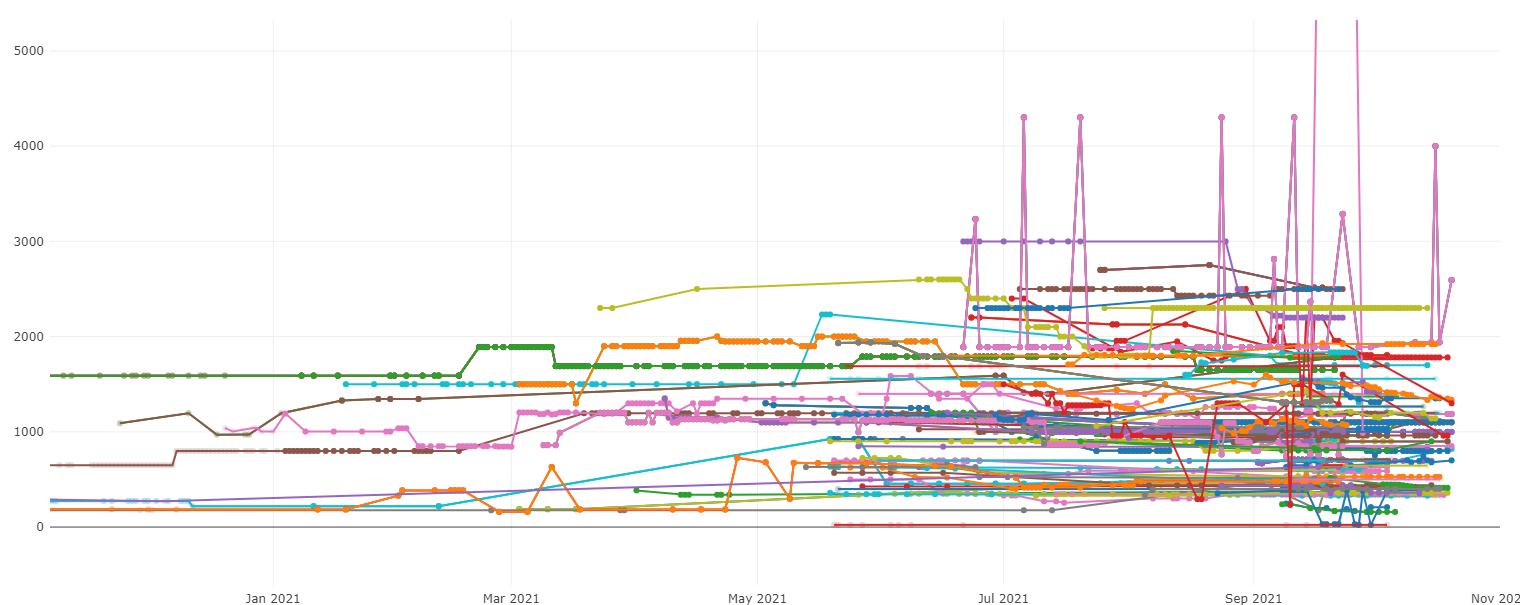
\includegraphics[width=\textwidth,height=7cm]{Hero} \\
    \caption{Historical card data for all GPUs collected} 
    \label{Fig:Hero} 
}

\begin{document}
\maketitle
\thispagestyle{empty}
\pagestyle{empty}


\begin{abstract}
    Digging through data to find new insights using old information is the fundamental pillar of data archaeology. For this Final Project, I have chosen to evaluate potential market price indicators of the GPU Market and draw insights as to when their prices may return to MSRP.
\end{abstract}

\section{Introduction}
Covid-19 has had a large impact on our lives. Throughout the year of 2020, many people could not attend work, leading to production, shipping, and ultimately availability and pricing issues of many products. These issues persist to this day although in many countries the restrictions leading to people not attending work have lifted. This projects attempts to gain insights as to when prices may return to normal for GPUs. 

\subsection{Objective}
For this project the number one objective is to find the top market indicators for GPU Pricing. This will be done by collecting large amounts of related data and performing Pearson Correlation Coefficient calculations between the collected data and historical GPU prices to find potential market indicators we can use to predict when prices may return to normal. Correlation information regarding all data will be collected, also allowing the direct comparison of Covid-19 and GPU prices, or potentially, numerically Covid-19's direct effect on the market price.

\subsection{Motivation}
This project was motivated by the recent spike in consumer electronic prices, ranging from televisions to computers. GPUs seem to have taken a particularly hard hit. Production rates have dropped for high-end hardware components as the yield decreases due to increased complexity of the architectures. Availability of GDDR5X-6X memory has decreased. On top of this, GPU manufacturing companies are still creating new products of previously unseen performance, further raising the base costs. Demand has skyrocketed as people begin to spend more times at their computers. With these factors combined, it's not uncommon to find GPUs marked up by as much as 10x. My personal GPU, the Nvidia GTX 1070, a five year old card, is currently trading for 42 percent more than what I bought it for. My motivation for this project is to hopefully gain insight into the future trading prices of cards as Covid-19 hopefully begins to recede.

\section{Data}
this section overviews each of the main sources of data, where the source was obtained, and the collection and cleaning processes.

\subsection{Selection of Cards}
The cards selected were based on the top 20 most popular cards on \cite{userBenchmark}, which generates these statistics from a combination of user voting, price, and performance. There is no corresponding scraper script for this task, the top 18 cards were simply saved in a json file manually. This list contains both pre-inflated and post-inflated GPU data.

Next, for each card, the top 10 most popular venders returned from a filtered search result on Honey.com were compiled. In all, 152 individual venders were collected.

\subsection{Historical GPU Prices Data}
The Historical GPU Prices were mined from Honey.com. There is no available public API for querying this information, so I created getter\_scripts/{getHoneyData getHoneyUrls}.py. These files find the honey URL endpoints which contain the GPU's historical price data and downloads them respectively.

\subsection{Covid-19 Data}
The covid-19 dataset was downloaded from \cite{covid}. It is a csv file containing a running count of covid cases throughout the world organized by country. This data was parsed, and the total running count for the world was extracted on a per-day basis.

\subsection{Google Trend Data}
The Google Trend dataset was downloaded via the getter\_scripts/getGoogleCardTrends.py script. This script utilyzes pytrend, a library for querying google trend data. For each card, the relevant trending data is saved on a per-day basis.

\subsection{GPU Spec Data}
GPU spec data was mined via getter\_scripts/getCardData.py which scrapes \cite{gpuSpecs} with BeautifulSoup. A sleuth of information is collected from each card, which is saved to a respective .json file.

\subsection{Software Data}
For this dataset, a csv file from kaggle (\cite{softwareData}) was downloaded containing the most popular (by number of sales) videogames since 1984. This file was parsed to only include games that made over 5 million dollars worldwide. 

\subsection{Cyrpto Trend Data}
Crypto trends were collected just as the Google Trend Dataset was collected. 

\subsection{Historical Crypto Prices Data}
Historical Crypto prices were collected from kaggle (\cite{cryptoHistory}) in csv format. In total, 23 different crypto coins and their price histories were parsed and recorded.

\section{Data Transformations}
The final form of all datasets is a dictionary keyed on dates (by day) with singular floating point values representing some measurable metric as the value. These dictionaries, after being processed, are cached and saved in a json file. This data is then loaded into the javascript application for further processing and interactive rendering of the datasets.

\section{Application}
To better visualize the collected data an application was created. In addition to visualizing, the application was also utilized to check for errors, find outliers, and validate results visually.

\subsection{Features}
Allows for every individual collected piece of downloaded data to be displayed on its own - or with any combination of selected datasets. 

If two (and only two) datasets are collected, their correlation coefficients are calculated and displayed. 

A "normalize" button was introduced to interpolate all data between the maximum and minimum values, to better show correlations between datasets.

A ranged input selector was also introduced to allow users to explore the data by correlation rankings in sorted order - highly negatively correlated datasets on the left, and highly positively correlated datasets on the right. When a user selects a value, the graph is updated to contain the respective datasets for viewing.

A snapshot functionality was introduced to allow pictures of the dataset to be taken. This functionality was used for all of the pictures used throughout this paper showing off the application.
\subsection{Visualizations}
%%%%%%%%%%%%%%%%%TODO%%%%%%%%%%%%%%%%%%%%%
Below are some visualizations taken from exploring the dataset using the application. 


\begin{figure}[h]
\centering
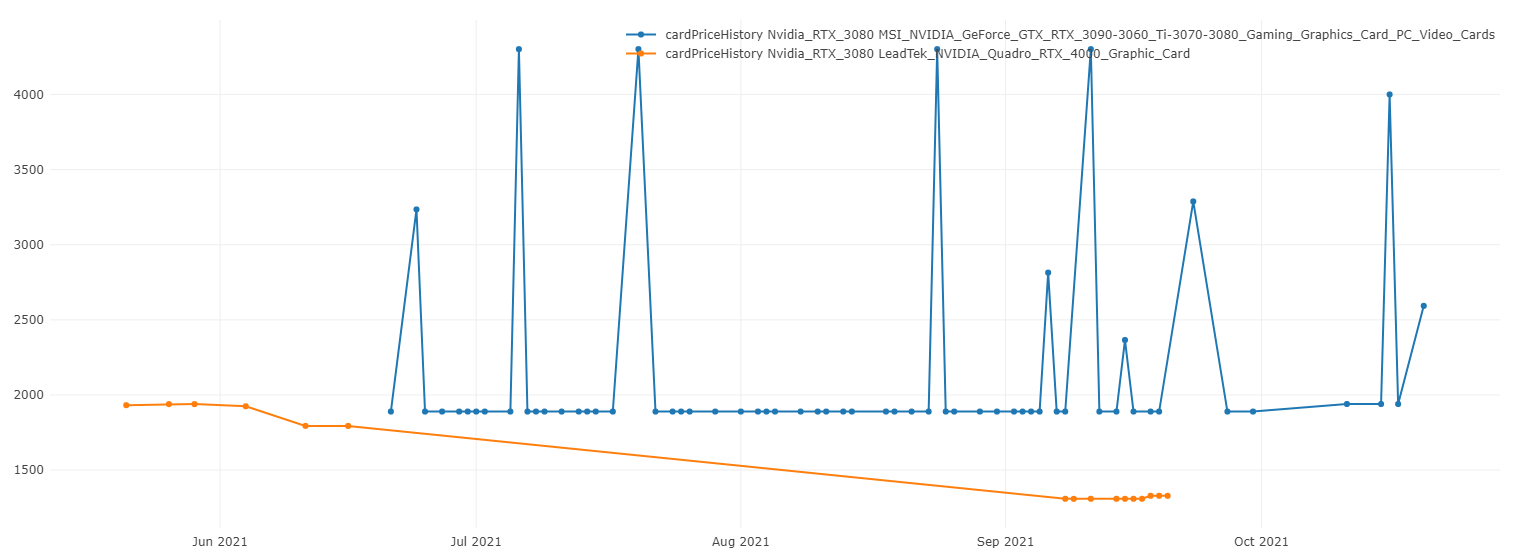
\includegraphics[width=0.4\textwidth]{3080-two-plot-example} 
\caption{An example of 2 plots being compared between two 3080 gpus over a similar time frame. The correlation coefficients will automatically be calculated and displayed in the application for the two selected datasets.}
\label{fig:plotExample}
\end{figure}

\begin{figure}[h]
\centering
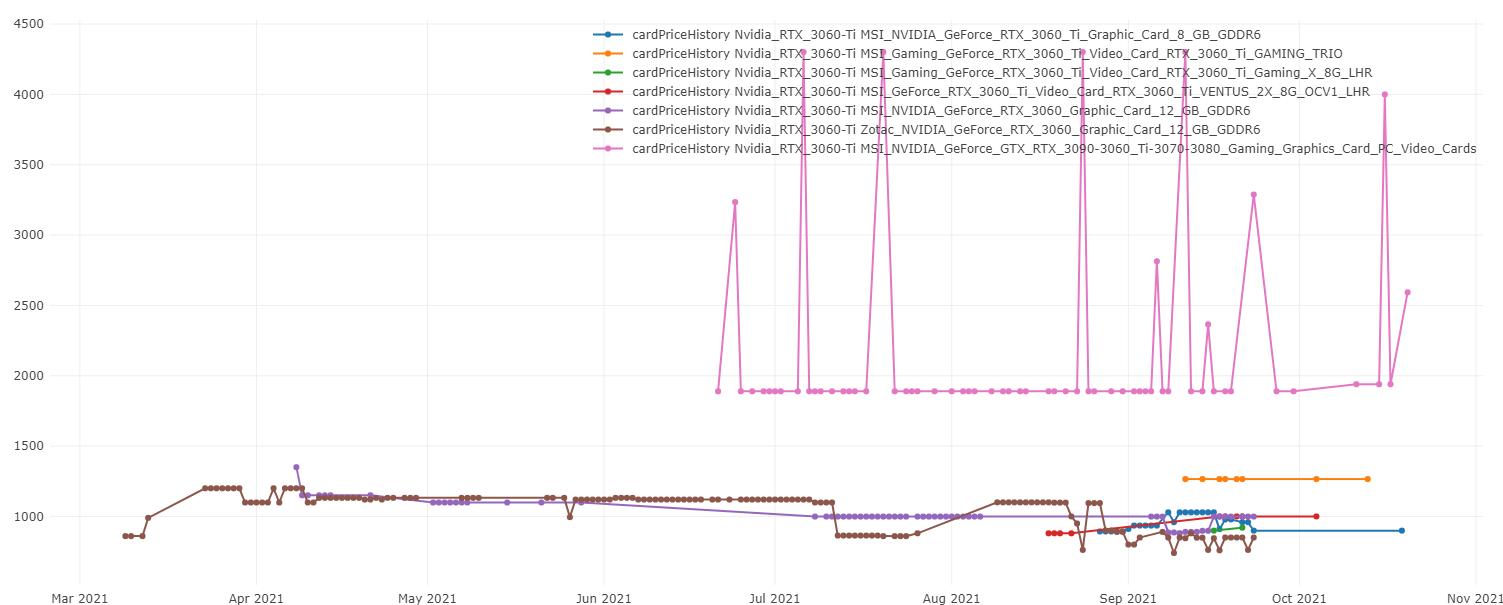
\includegraphics[width=0.4\textwidth]{3060-ti} 
\caption{A plot showing all of the raw scraped 3060-ti data}
\label{fig:3060_ti}
\end{figure}

\begin{figure}[h]
\centering
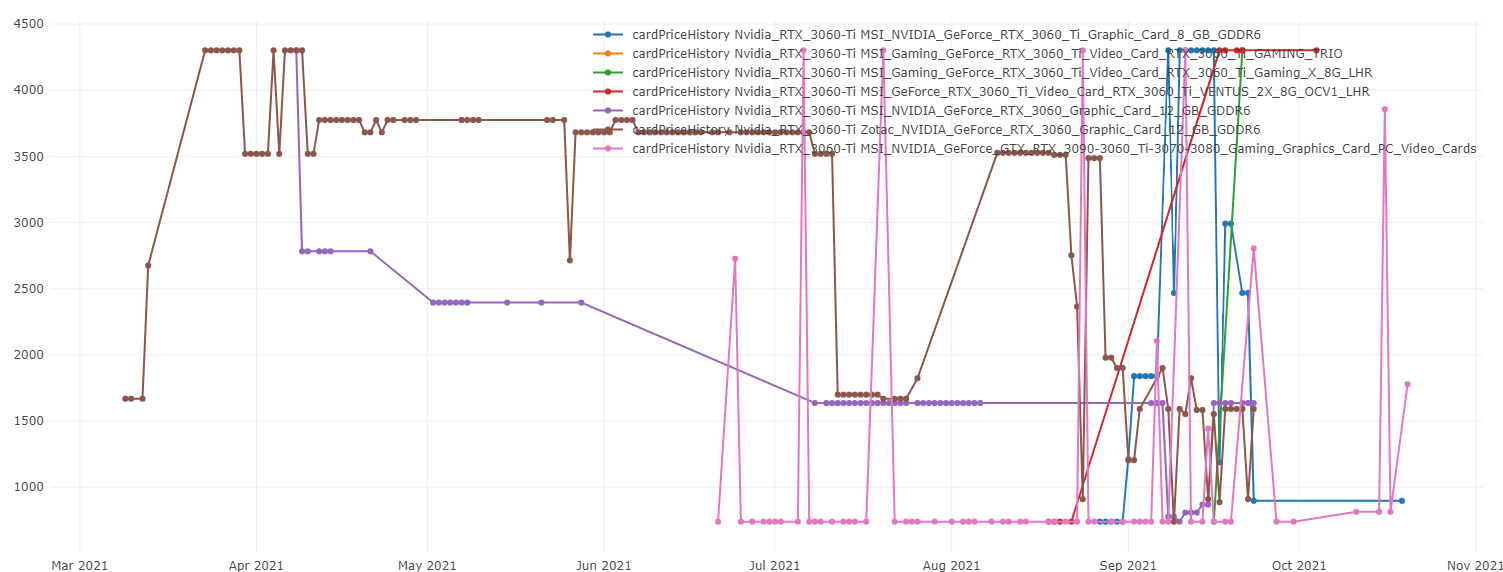
\includegraphics[width=0.4\textwidth]{3060-ti_normalized} 
\caption{The same plot as figure \ref{fig:3060_ti}, but with the normalized setting applied}
\label{fig:3060_ti_normalized}
\end{figure}

\section{Insights}
Variables such as GPU pricing may be unpredictable, but there may exist high correlation coefficients to outside factors that are predictable. Although correlation is not causation, things do not tend to fall out of correlation when associated for long durations of time. We can assume with relative assurance that one day covid will end, one day newer, better performing GPUs will be released, and one day a new software will be released. With these insights, given constant correlations, we can predict future GPU prices of existing cards.

\subsubsection{Relation to Crypto}
\begin{figure}[h]
\centering
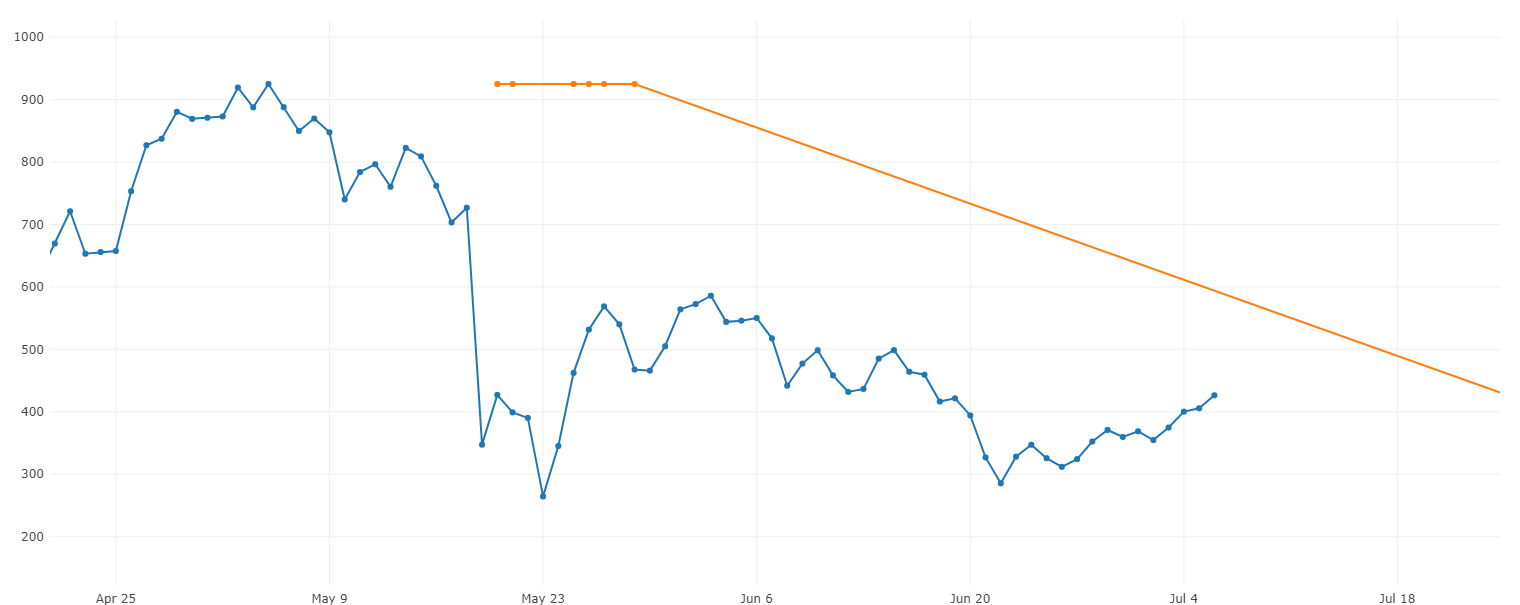
\includegraphics[width=0.4\textwidth]{Zotac_1060_Coin_uniswap} 
\caption{normalization on comparing a Zotac 1060 to CryptoCoin UniSwap}
\label{fig:Zotac_1060_Coin_uniswap}
\end{figure}
There are very strong positive correlations between most GPUs and the majority of Crypto stock prices. Crypto prices have recently steeply dropped, and with it, several GPU vendor's prices have as well. The result drop is still well above MSRP, but is several times closer to MSRP than before the drop for most observed cards containing this correlation. This suggests the market is actively recovering, despite falling Crypto prices. This correlation also makes sense - As crypto prices fall, there is less demand on GPU resources as people become disinterested in mining and begin selling their cards for cheaper prices, and no longer scalp the market for high-end cards.

\subsection{Card to Card Relations}
Cards of a similar league (release date & specs) tend to be positively correlated. The more similar the card, the higher the correlations tend to be. This makes sense, as if the cards became too disjointed in price, all consumers would only buy cards from one vendor. In Microeconomics terms, these products are said to be "related".

Cards of dissimilar leagues tend to be negatively correlated, again, the more dissimilar the card, the higher the correlation. This makes sense, as older, weaker, more dissimilar cards become lower in price as newer, more powerful cards come out and become higher in price. 

\subsection{Card to Covid Relations}
\begin{figure}[h]
\centering
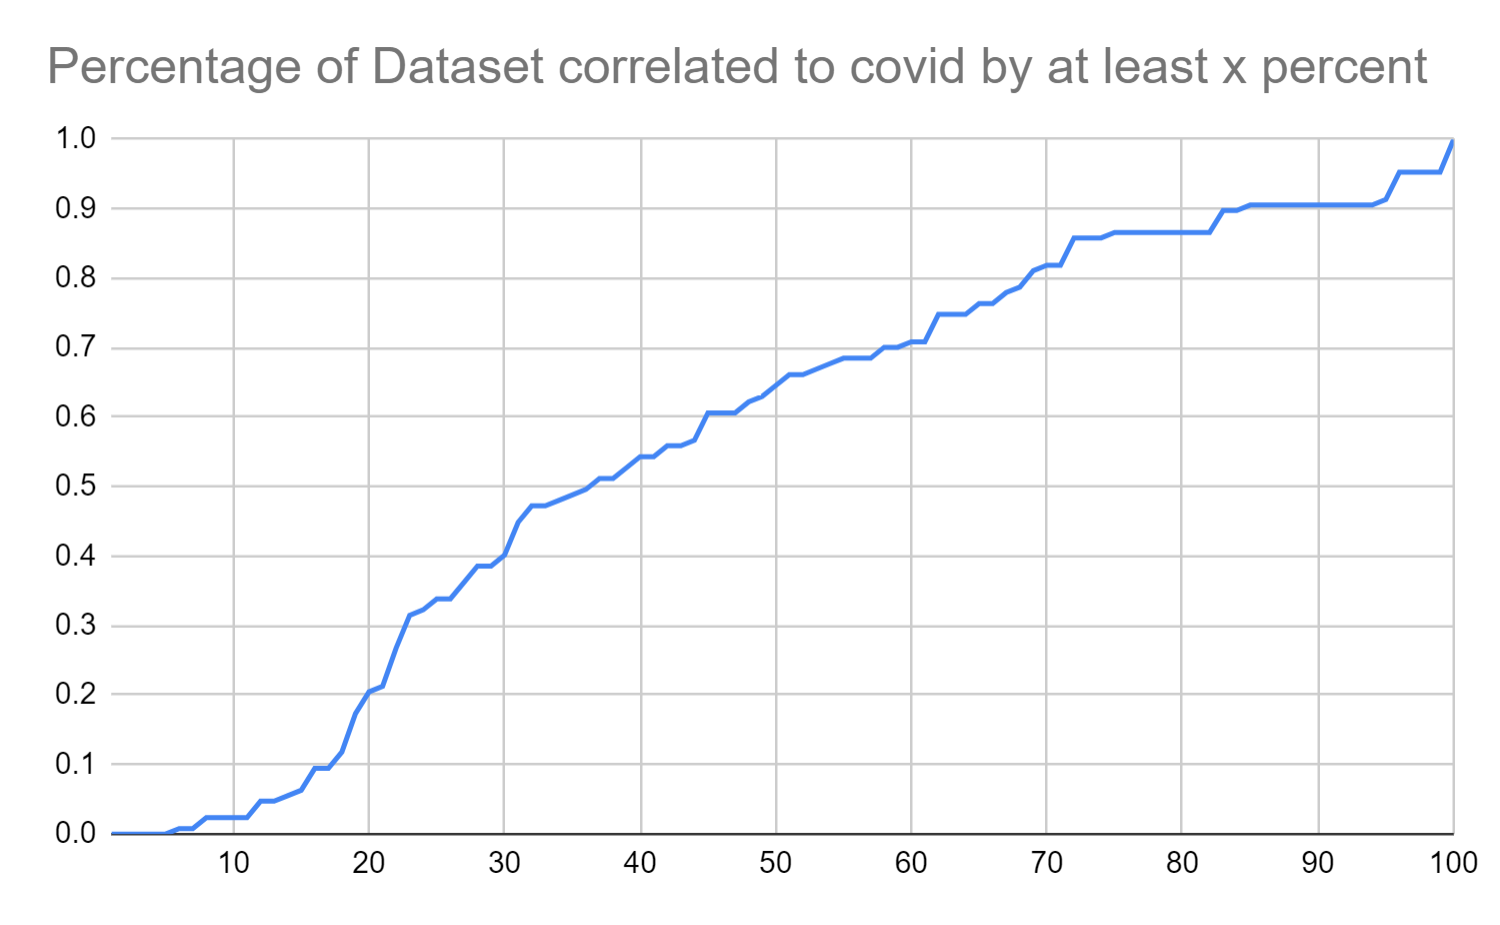
\includegraphics[width=0.4\textwidth]{covid_correlations }
\caption{The magnitude of correlations (x-axis) vs what percentage(y-axis) cards fit that criteria}
\label{fig:covid_correlations}
\end{figure}
As can be seen in figure \ref{fig:covid_correlations}, 50\% of the data is of 35\% correlations or greater. The outward bow of the curve suggests there is a preference for data to be more strongly correlated than weakly correlated to Covid. This makes sense, as the Covid dataset is a relatively simple monotonically increasing series, so cards that either fall significantly in price or rise significantly in price will be more greatly correlated with covid.

\section{Challenges}
\subsection{Discrete Time Series Events}
The largest challenge encountered was calculating the Pearson correlation coefficients for non-time-series data. This includes the GPU Spec and Software datasets. Since these "events" in time are singular and non-continous, a continuous analogue was created for both. I refer to these continuations as the "hype trend". A time of 1 is assigned to the day of the event. A linear equation is modeled from value 0 to 1 from 80 days before the event to the event epoch. Another linear equation is also modeled from the time of the epoch to the current day, from 1 to 0. This model will show that hype will begin building 80 days before the event occurs, and hype slowly decreases throughout the life of the event. The exact values chosen do not matter much (i.e the magnitude of the hype being 1) as only the direction in change of values from one time step to the next is utilized when calculating the Pearson correlation coefficient. This provides a nice analogue for discrete events - as the event epoch date nears, positive correlations are formed, and as the date is exceeded, negative correlations are formed.

\subsection{Missing Data}
Since the Pearson correlation coefficients are computed per-day, every day must be included in every dataset. In most datasets there are date ranges missing for various reasons (no one bought GPUs that day, Honey did not track data for that day, non business day, etc). and these values must be filled. Several valid choices can be made including filling with 0's, linearly interpolating between known values, or copying the last known value. I chose the last option for my implimentation.

\subsection{RAM usage and dataset size}
Originally, the application was written in Python utilizing MatPlotLib as the visualization/interactivity tool. This ended up being too slow, especially in Jupyter Notebooks, which took several minutes to display a single selected dataset. To combat this, I remade the application in Javascript as a Front End Web Application available to anyone at \cite{jhammer3}

\section{Results}
A set of all correlations between all collected datasets and all collected historical GPU prices has been generated. This file served as the beginning of further exploration of the application, and generation of key insights and future predictions. This file is available at /correlations.txt. It is in a simple format.

The full application is available at all times at \cite{jhammer3}. 

\section{Future Work}
Future work could include making predictions using the information given by training autoencoders on the given data. This could be made more accurate by including all datasets in the training portion, and in the prediction/generation portion we could assume several factors, such as covid cases increasing. I chose not to implement this though as this predictions would not be accurate, as they are only based on past data, not potential future happenings, making them at best very inaccurate, but a cool toy nonetheless. 

\section{Conclusion}
In this project I have shown that there are correlations between GPUs and several outside factors that may play a "market indicator" role. If we are to assume that these are accurate market indicators, then GPU prices should decline as the positively correlated indicators decline, or decline as negative correlated indicators increase.

\begin{thebibliography}{99}

\bibitem{jhammer3} 1. https://www.web.eecs.utk.edu:\~/jhammer3/fdac21/ 

\bibitem{cryptoHistory} 2.  https://www.kaggle.com/sudalairajkumar/cryptocurrencypricehistory

\bibitem{softwareData} 3.  https://www.kaggle.com/gregorut/videogamesales/download/ OExKsLPk1MffQwx39Ex4\%2Fversions\%2FHrmHcMK3ZvGhoCopnQhB\% 2Ffiles\%2Fvgsales.csv?datasetVersionNumber=2

\bibitem{gpuSpecs} 4. https://www.techpowerup.com/gpu-specs/

\bibitem{userBenchmark} 5. https://gpu.userbenchmark.com

\bibitem{covid} 6. https://github.com/CSSEGISandData/COVID-19/ blob/master/csse\_covid\_19\_data/csse\_covid\_19\_time\_series/ time\_series\_covid19\_confirmed\_global.csv

\end{thebibliography}


\addtolength{\textheight}{-12cm}   % This command serves to balance the column lengths
                                  % on the last page of the document manually. It shortens
                                  % the textheight of the last page by a suitable amount.
                                  % This command does not take effect until the next page
                                  % so it should come on the page before the last. Make
                                  % sure that you do not shorten the textheight too much
\end{document}